\section{Validierung}\label{sec:Validierung}
In diesem Kapitel wird zuerst der Versuchsaufbau erklärt. Danach werden die einzelnen Versuche und deren Erkenntnis erläutert.\\
Drehmoment-Drehzahl\\
hohe Drehzahl unter Last\\
Leistung-Temperatur\\
Spannungsabfall\\
Temperatur\\
Steuerkurve\\
max Drehzahl bei variabler Spannung\\
max Drehmoment bei variabler Spannung\\

\subsection{Versuchsaufbau}\label{subsec:Versuchsaufbau}
Für den Versuchsaufbau wurde ein BLDC-Motor mit einer asynchronen Maschine gekoppelt welche über einen Frequenzumrichter angesteuert wird und netzspeisefähig ist. Die ASM diente bei den nachfolgenden Versuchen als Last. Damit verschiedene Betriebszustände gemessen werden konnten, wurden Drehzahl auf seiten des BLDC und Leistung auf Seiten der ASM ausgewertet. Die mitgelieferte Software des BLDC-Motors diente zur Überwachung der Motoren-, und Controller Temperatur.


\subsection{Drehmoment bei variabler Drehzahl}\label{subsec:DrehmomentDrehzahl}
Um zu bewiesen, dass der Motor die erforderliche Leistung erbringen kann, wurde das Drehmoment in Abhängigkeit der Drehzahl untersucht.

% dieser Teil eventulle in den Hartwareteil verschieben und nur darauf Referenzieren
Bei einem minimalen mechanischen Wirkungsgrad von 0.8, einem 1:16 Getriebe und einem Trommeldurchmesser von 80cm, muss der Motor ein konstantes Drehmoment von 32Nm liefern. 

Die Bedingungen, mit welcher der Versuch durchgeführt wurde, können der Tabelle \ref{tab:Drehmoment/Drehzahl} entnommen werden.

\begin{table}[H]
\centering
\begin{tabular}{C{4cm} C{4cm} C{3cm}} 
\multicolumn{3}{c}{\textbf{Versuchsbedingungen}} \\
{Messgrösse}& {Bedingung} & {Wert}\\ \hline\hline 
Spannung (DC)   & nachgeregelt &   96 V     \\
Strom (DC)   & gemessen &   37.8-128 A     \\
Leistung (AC)   & gemessen &   1702-8870 W    \\
Drehzahl   & variiert &   614-2954 RPM    \\
Drehmoment-Sollwert   & nachgeregelt &   32 Nm    \\
Motor-Temperatur   & vernachlässigt &   -    \\
Controller-Temperatur   & vernachlässigt &   -    \\
\end{tabular}
\caption{Versuchsbedingungen Drehmoment/Drehzahl-Versuch}\label{tab:Drehmoment/Drehzahl}
\end{table}

Das Drehmoment an der Welle des BLDC-Motors wird mithilfe der Formel (FORMEL IN HARWARE/GRUNDLAGEN) über die Leistung und der Drehzahl des Motors ermittelt. Diese Kurve ist in der Abbildung \ref{fig:drehmoment/drehzahl} (blaue Kurve) ersichtlich. Da die asynchrone Maschine ebenfalls nicht ideal arbeitet, wird bei dieser einen Wirkungsgrad von 90\% angenommen (rote Kurve).

\begin{figure}[H]
	\centering
	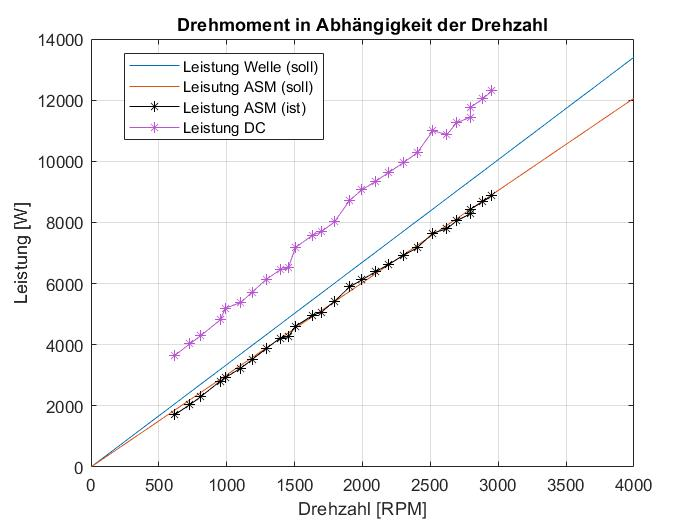
\includegraphics[width=0.8\linewidth]{drehmoment_drehzahl.jpg}
	\caption{Drehmoment in Abhängigkeit der Drehzahl}\label{fig:drehmoment/drehzahl}
\end{figure}

Bei diesem Versuch ist ersichtlich, dass es möglich war, die erforderliche Leistung (schwarze Punkte) im Drehzahlbereich zwischen 600 und 3000 RPM zu erreichen. Die aufgenommene Leistung auf der DC-Seite (violette Punkte) ist dabei proportional zur abgegebenen Leistung angestiegen und erreicht bei 3000 RPM einen Wert von über 12kW.

In der Abbildung \ref{fig:drehmoment/StromSpannung} sind die Spannung, der Strom und die Sollwertvorgabe für die Ansteuerung während des Versuchs ersichtlich. Die Spannung wurde auf $96V_{DC}$ nachgeregelt (blaue Punkte), damit diese für den Versuch konstant blieb. Der Strom (rote Punkte) und der Sollwert für die Ansteuerung (orange Punkte) wurden ebenfalls während des Versuchs dokumentiert.


\begin{figure}[H]
	\centering
	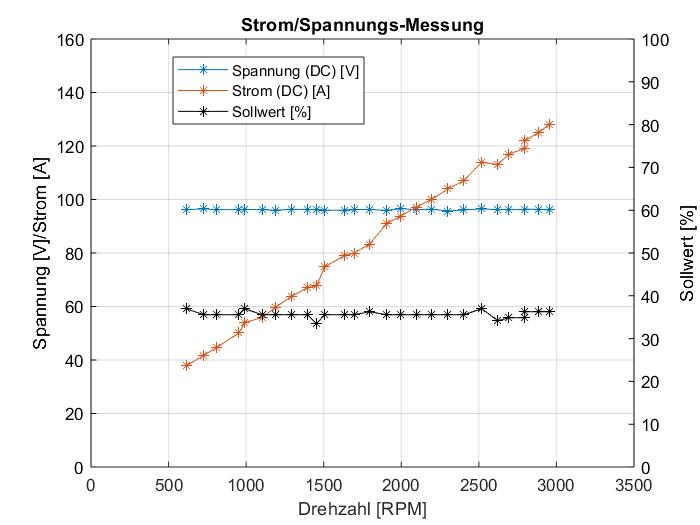
\includegraphics[width=0.8\linewidth]{drehmoment_StromSpannung.jpg}
	\caption{Spannung und Strom während des Drehmomentversuchs}\label{fig:drehmoment/StromSpannung}
\end{figure}

%Welcher graue Transformator? Verweis auf ein Versuchsaufbau Bild?
Da der graue Transformator nur für einen Strom von 95A konzipiert ist, was bei der verwendeten B6-Brückenschaltung einem Strom (gemäss Formel \ref{eq:B6}) von rund 128A im DC-Zwischenkreis entspricht, konnte der Versuch nicht bis 3800 RPM durchgeführt werden. Der Strom kann mit guter Näherung als linear zur Drehzahl bei gleichbleibendem Drehmoment betrachtet werden. Dadurch ist ersichtlich, dass bei 3800 RPM ein Strom von ca. 160A benötigt wird. Dies Stromstärke deckt sich auch mit dem Wert im Datenblatt des Motors (REFERENZ AUF DATENBLATT).

Bei diesem Versuch ist ebenfalls ersichtlich, dass die Sollwertvorgabe über den Drehzahlbereich nur kleine Abweichungen hat und daher in guter Näherung als konstant betrachtet werden kann.



\subsection{Leistungsabhängigkeit der Temperatur}\label{subsec:Leistung/Temperatur}
Da der BLDC-Motor eine sehr kleine Bauform für seine Grösse hat, unterliegt dieser grossen Temperaturschwankungen. Hierbei wird untersucht, wie sich die Temperatur bei konstantem Sollwert auf die Leistung auswirkt. Die Versuchsbedingungen können der Tabelle \ref{tab:Leistung/Temperatur} entnommen werden.


\begin{table}[H]
	\centering
	\begin{tabular}{C{4cm} C{4cm} C{3cm}} 
		\multicolumn{3}{c}{\textbf{Versuchsbedingungen}} \\
		{Messgrösse}& {Bedingung} & {Wert}\\ \hline\hline 
		Spannung (DC)   & nachgeregelt &   96 V     \\
		Strom (DC)   & gemessen &   106-112 A     \\
		Leistung (AC)   & gemessen &   7330-7820 W    \\
		Drehzahl   & konstant &   2500 RPM    \\
		Drehmoment-Sollwert   & konstant &   32 Nm    \\
		Motor-Temperatur   & gemessen &   30-100 °C    \\
		Controller-Temperatur   & vernachlässigt &   -    \\
	\end{tabular}
	\caption{Versuchsbedingungen Leistung/Temperatur-Versuch}\label{tab:Leistung/Temperatur}
\end{table}

Wie in der Abbildung \ref{fig:Leistung/Temperatur} ersichtlich ist, nimmt die Leistung bei zunehmender Temperatur ab. Die Leistung verringerte sich bei einer Motor-Temperatur von 100°C um ca. 6\% gegenüber einer Temperatur von 30°C. Die Leistungsabnahme ist dabei in guter Näherung linear zur Temperatur.

\begin{figure}[H]
	\centering
	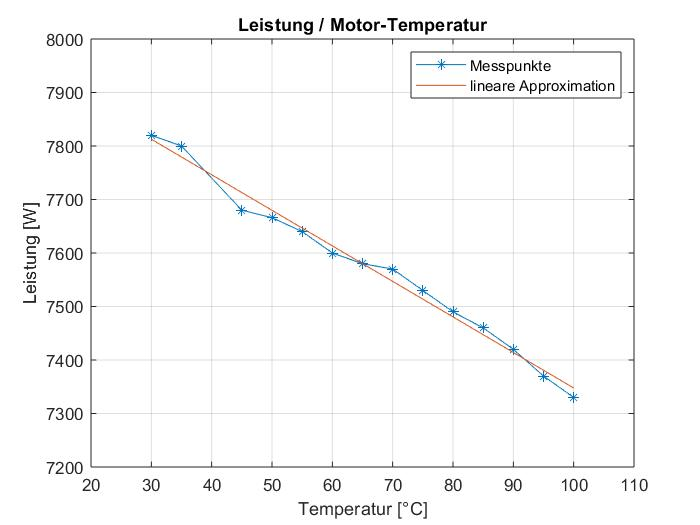
\includegraphics[width=0.8\linewidth]{LeistungTemperatur.jpg}
	\caption{Einfluss der Erwärmung auf die Leistung}\label{fig:Leistung/Temperatur}
\end{figure}

\subsection{Leistungsverhalten bei Spannungsabfall}\label{subsec:LeistungSpannungabfall}
Bei diesem Versuch wird das Verhalten des Controllers bei einem Spannungsabfall untersucht. Dabei wurde sowohl die Leistung der ASM (Abbildung \ref{fig:Spannungsabfall} rechts) als auch der Strom des Controllers (Abbildung \ref{fig:Spannungsabfall} links) in Abhängigkeit zur Spannung des Controllers gemessen. Der Sollwert wurde während des gesamten Versuchs konstant auf 35.5\% gehalten, was dem Wert des Drehmomentversuches (\ref{subsec:DrehmomentDrehzahl}) entspricht. Dieser Versuch wurde zuerst mit 1500 RPM (blaue Punkte) und danach nochmals mit 2000 RPM (rote Punkte) durchgeführt.

\begin{figure}[H]
	\centering
	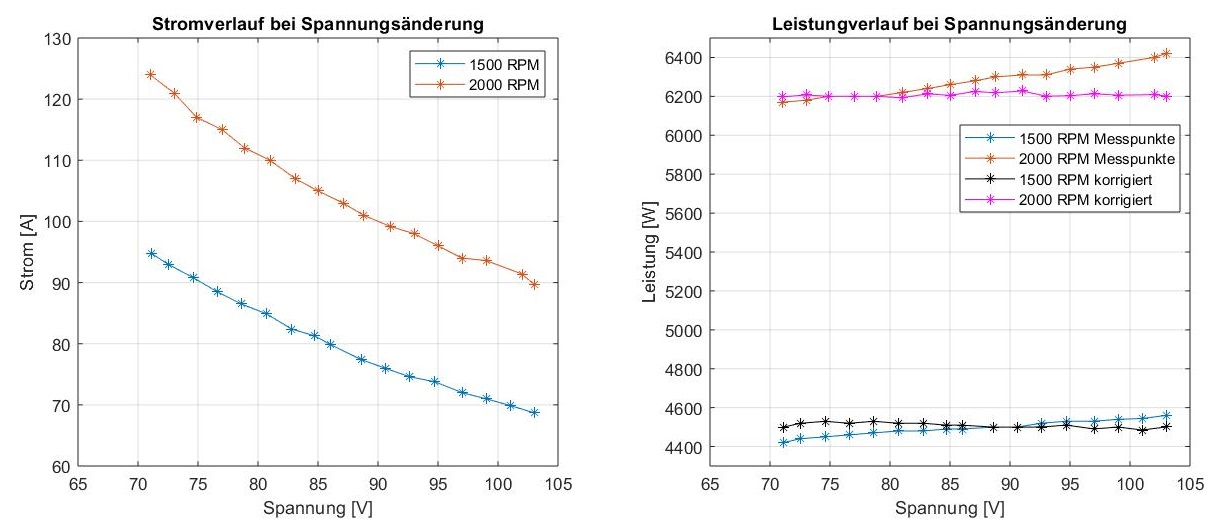
\includegraphics[width=1\linewidth]{Spannungsversuch.jpg}
	\caption{Leistungs- und Stromverlauf bei Spannungsabfall}\label{fig:Spannungsabfall}
\end{figure}

Aus diesem Versuch ist ersichtlich, dass der Controller bei einem Spannungsabfall und konstantem Drehmomentsollwert die Leistung nachregelt indem der Strom erhöht wird. Während die Spannung um 32\% abfällt, nimmt der Strom um ca. 28\% zu. Dabei verhält sich die Stromzunahme linear zum Spannungsabfall. Die Leistung nimmt dabei lediglich um ca. 4\% ab.

Dadurch kann der Schluss gezogen werden, dass der Spannungsabfall keinen grossen Einfluss auf die Leistung hat. Durch die erhöhte thermische Belastung bei grösseren Ströme ist eine möglichst grosse Spannung jedoch erstrebenswert.

\subsection{Maximale Drehzahl bei variabler Spannung}\label{subsec:DrehzahlSpanungsabfall}
In diesem Versuch wird das Verhalten des Motors bei Unterspannung untersucht. Dabei wurde der Sollwert für das Drehmoment auf dem Maximum gehalten, während der Motor im Leerlauf dreht. Die Spannung wird dabei langsam erhöht. Die Drehzahl ist dabei elektronisch im Controller auf 3800 RPM begrenzt, da die asynchrone Maschine keine höheren Drehzahlen zulässt und ist in nachfolgender Abbildung \ref{fig:maxDrehzahl} graphisch dargestellt.

\begin{figure}[H]
	\centering
	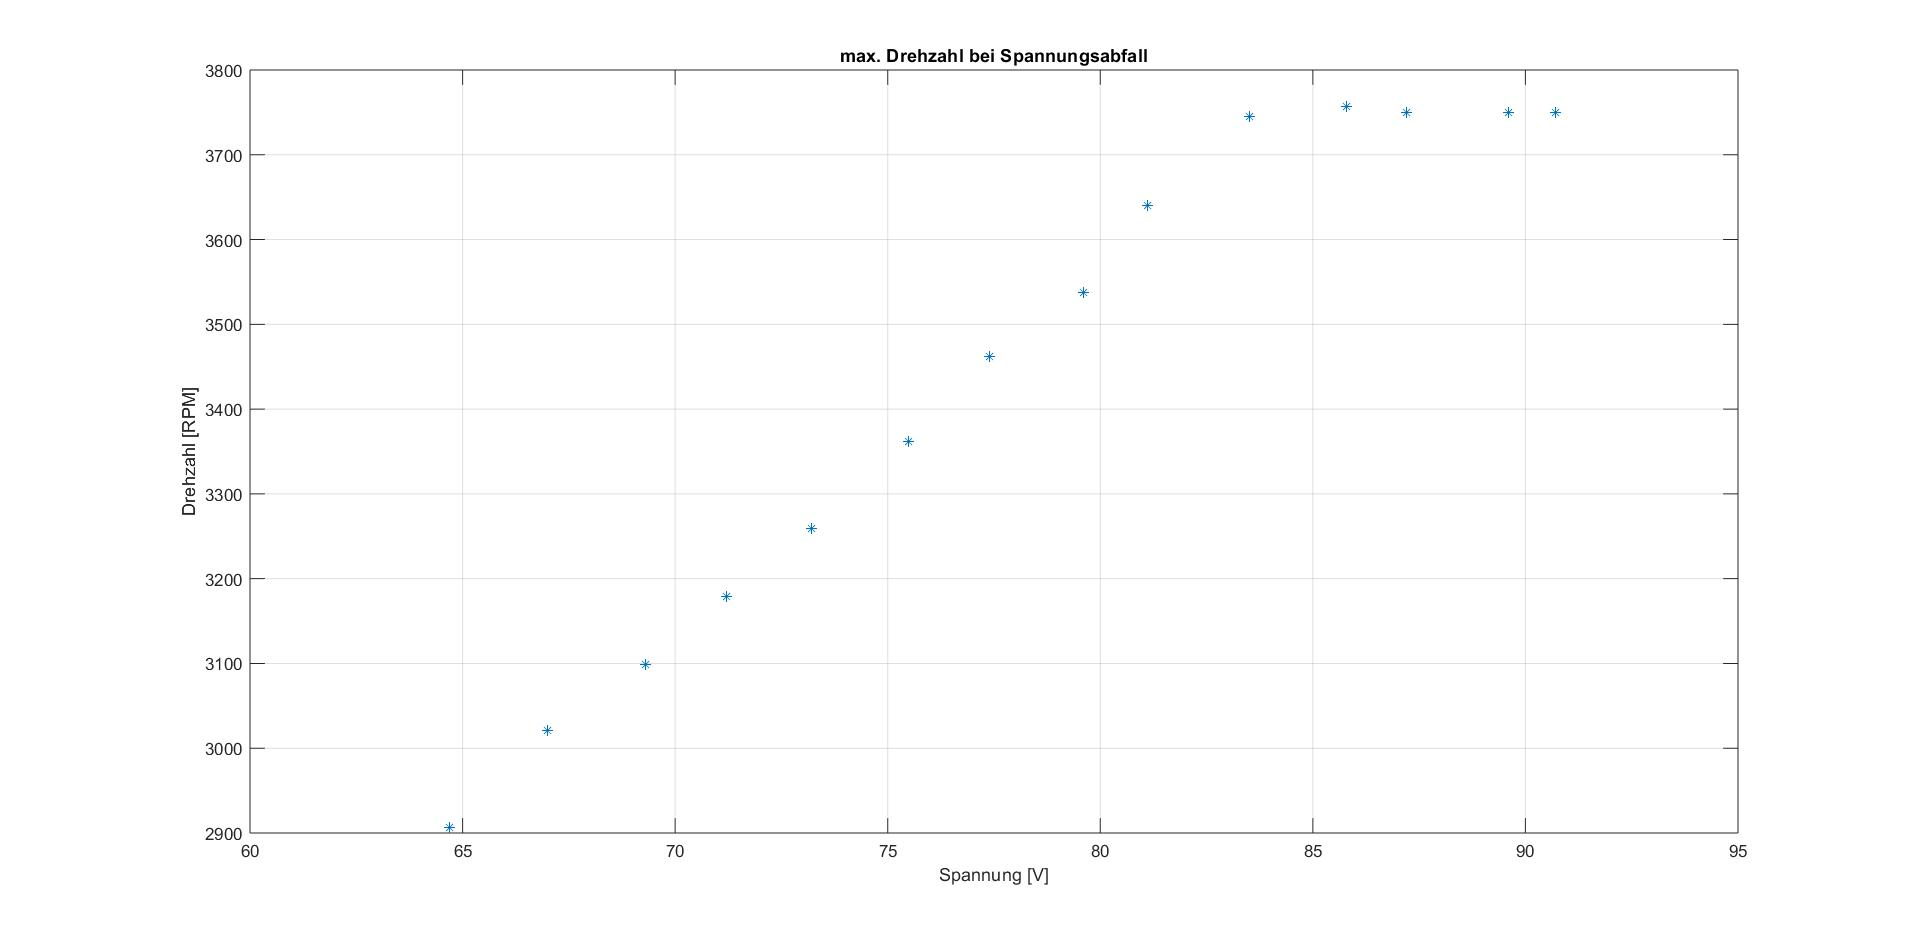
\includegraphics[width=0.8\linewidth]{maxDrehzahl.jpg}
	\caption{Maximale Drehzahl}\label{fig:maxDrehzahl}
\end{figure}

Bei diesem Versuch hat sich gezeigt, dass die Versorgung mindestens 84V bringen muss, damit der BLDC-Motor 3800 RPM erreichen kann. Weiter ist ersichtlich, dass die Leerlaufdrehzahl ca. 45 RPM pro Volt sinkt.


\subsection{Maximale Leistung bei variabler Spannung}\label{subsec:LeistungSpannungsabfall}
In diesem Versuch wird die maximale Leistung bei einem Spannungsabfall untersucht. Da die asynchrone Maschine nicht für 3800 RPM ausgelegt ist, wurde dieser Versuch bei einer konstanten Drehzahl von 3600 RPM gemessen. Wie im vorhergehenden Versuch, wurde das Drehmoment aufs Maximum eingestellt, während die Spannung langsam erhöht wurde.


\begin{figure}[H]
	\centering
	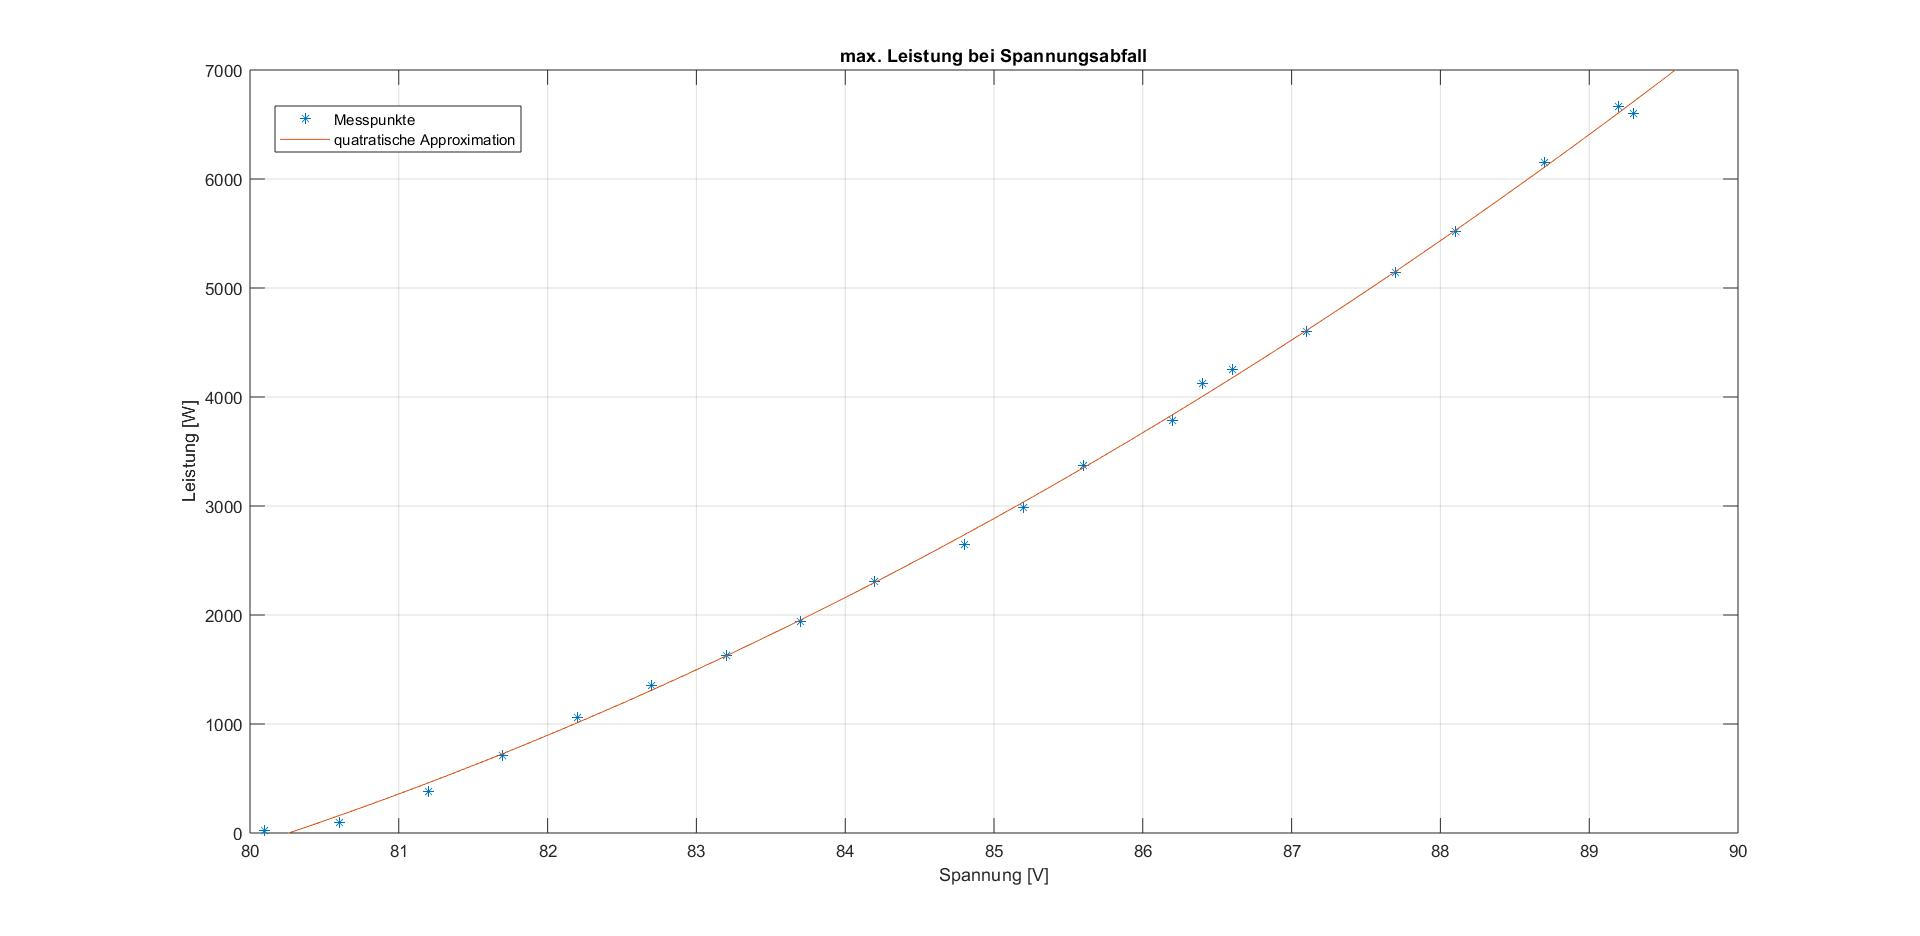
\includegraphics[width=0.8\linewidth]{maxLeistung.jpg}
	\caption{Maximale Leistung}\label{fig:maxLeistung}
\end{figure}

Unter der Annahme, dass zwischen der maximalen Leistung und der Spannung ein quadratischer Zusammenhang besteht (rote Approximation), ist anzunehmen, dass die maximale Leistung bei 3600 RPM und Nennspannung (96V) bei 15kW liegt. Hierbei ist jedoch anzumerken, dass die effektive Leistung an der Welle des BLDC-Motors ca. 10\% höher ist, da diese auf der elektrischen Seite der asynchronen Maschine gemessen wurde.

\subsection{Temperaturversuch}
Um einen Einblick in das Temperaturverhalten des Motors zu erlangen, wurde in diesem Versuch die Erwärmung in Abhängigkeit der Drehzahl bei konstantem Moment gemessen. Die Messung erfolgte bei einer Drehzahl von 1550 RPM und bei 2550 RPM, und einem jeweiligen Drehmoment von 32Nm. Die Starttemperatur des Motors lag jeweils bei ca. 60°C und wurde solang betrieben, bis er eine Betriebstemperatur von 100°C erreicht hatte.


\begin{figure}[H]
	\centering
	\includegraphics[width=0.8\linewidth]{Temperatur.jpg}
	\caption{Erwärmung}\label{fig:Temperatur}
\end{figure}


Da die Leistung sowohl vom Drehmoment als auch von der Drehzahl abhängig ist, wurde beim Versuch bei 2550RPM eine höhere Leistung und somit auch ein grösserer Strom erzielt. Aus diesem Grund ist die Erwärmung des Motors bei höheren Drehzahlen dementsprechend grösser. Anhand der beiden Versuchen gehen wir davon aus, dass der BLDC-Motor ca. 5 Minuten unter Vollast betrieben werden kann, bis er die 100°C erreicht. Es gilt zu beachten, dass der Motor eine Betriebstemperatur von 110°C zulässt, wodurch eine Reserve von 10°C gegeben ist.
 